\chapter{The viscous cylinder}
The flow around a viscous cylinder has been approached by many papers both analytically \todo{wirklich?} and numerically, e.g. \todo{literatur}, though very few numerical approaches use a \gls{rkdg} method combined with immersed boundaries. In order to verify the \gls{bosss} code with immersed boundaries not only for the Euler equations as we did in chapter \ref{eulerVerification} but also for the viscous case we will now consider different Reynolds numbers for the steady and unsteady flow and compare our results to those of other studies.

\section{Theory}
	The flow around a viscous cylinder can be divided into different sections depending on the flow specific Reynolds number. The first section applies for Reynolds numbers $0 < \text{Re} < 40-50$ characterised by a laminar steady flow. In that regime a recirculation region with two symmetric vortices with opposite directions is comprised by the wake. The flow can be described using the wake separation length $W^*$.\\\\
	\begin{figure}[htp]
		\centering
		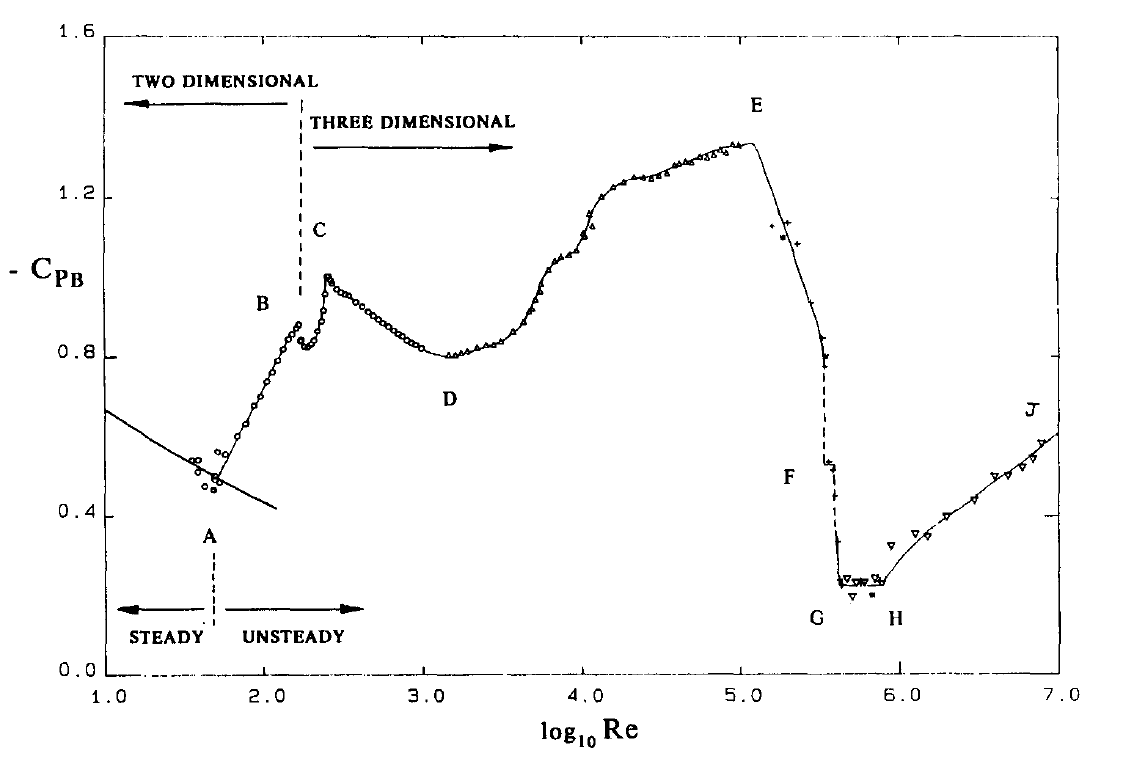
\includegraphics[height=8cm]{overviewCylinderReynolds_Williamson.PNG}
		\caption{Overview of Base Suction Coefficients over Reynolds Number \todo{Quelle}}
		\label{fig:overview}
	\end{figure} 
	The second section contains all other Reynolds number $\text{Re}> 40-50$ and thus describes the unsteady flow. It can be subdivided in several subsections:
	\begin{description}
		\item[$40-50 < \text{Re} < 190$] laminar vortex shedding,
		\item[$190 < \text{Re} < 260$] 3-D wake-transition regime,
		\item[$260 < \text{Re} < 1000$] increasing disorder in the fine-scale three dimensionalities,
		\item[$1000 < \text{Re} < 200000$] shear layer transition regime,
		\item[$200000 < \text{Re}$] critical transition, supercritical regime and post-critical regime.
	\end{description}
	
	As we will only discuss Reynolds numbers up to $\text{Re} = 200$ the important phases for us are the laminar steady regime and the laminar vortex shedding. At around $\text{Re} = 190$ the three dimensionality of the system has an incrementing influence on the flow; for we only analyse the 2-D model of the experiment we stop at $\text{Re} = 200$ expecting slight deflection in our results.
	
	\subsection{The Laminar Steady Regime}
	
		\begin{figure}[htp]
			\centering
			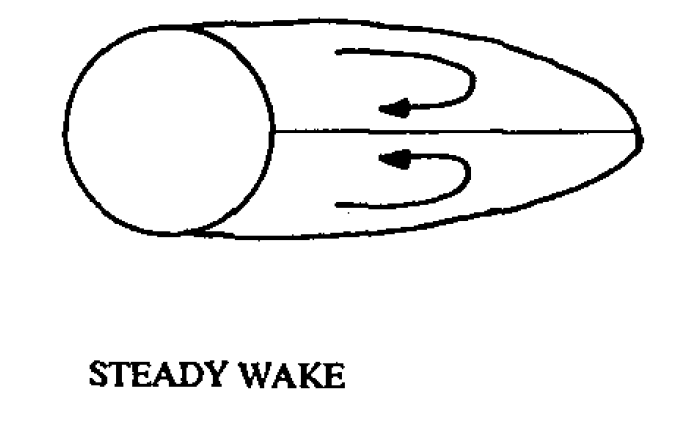
\includegraphics[height=4cm]{steadyFlow_Williamson.PNG}
			\caption{Recirculation Region \todo{Quelle}}
			\label{fig:steady}
		\end{figure}
	\subsection{Laminar Vortex Shedding}
	
		\begin{figure}[htp]
			\centering
			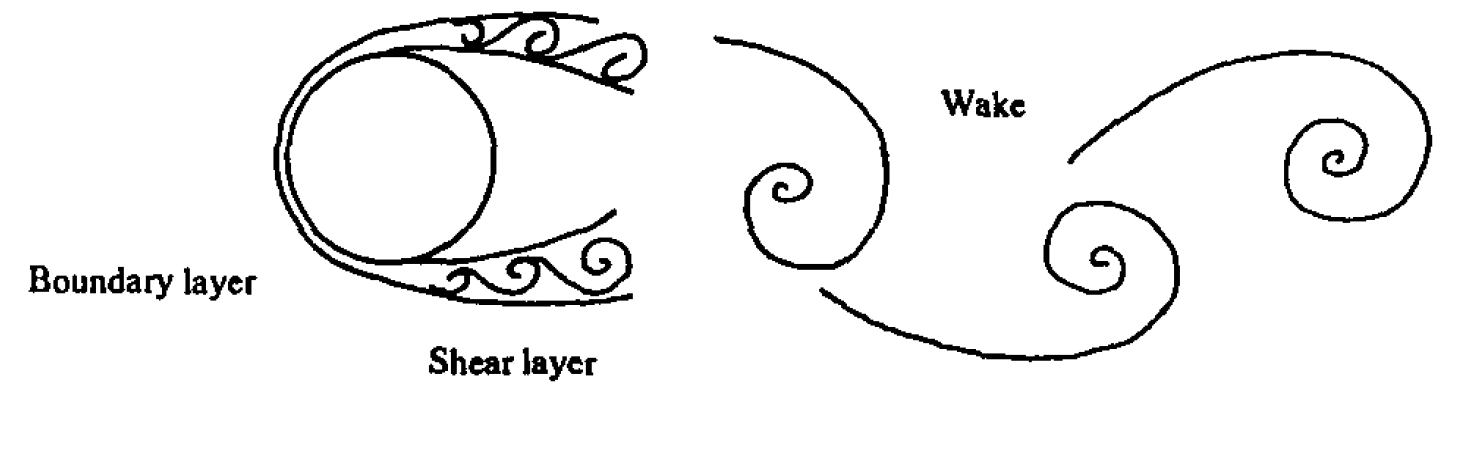
\includegraphics[height=4cm]{unsteady_Williamson.PNG}
			\caption{Karmán Vortex Street \todo{Quelle}}
			\label{fig:unsteady}
		\end{figure}
		
\section{Simulations}
	In this section we will compare the lift and drag coefficients at different Reynolds numbers and mesh sizes at a constant agglomeration threshold of $0.1$, different polynomial degrees of 1, 2 and 3 and meshes of $32 \times 32$, $64 \times 64$ and $128 \times 128$ cells. The different simulation properties will be abbreviated as DG $+$ \textit{polynomial degree} $+$ MP $+$ \textit{number of cells per direction}, eg DG2MP64 for a simulation with polynomial degree 2 and $64 \times 64$ cells.\\
	 The drag and lift coefficients $C_D$ and $C_L$ are defined as
	\begin{align}
		C_D = \dfrac{d}{q_\infty L_\infty} \\
		C_L = \dfrac{l}{q_\infty L_\infty}
	\end{align}
	with the dynamic pressure $q_\infty = \dfrac{1}{2} \rho_\infty V_\infty^2$. For we set $L_\infty = \rho_\infty = V_\infty = 1$ in our boundary and initial conditions, we can assume
	\begin{align}
		C_D = 2 \cdot d \\
		C_L = 2 \cdot l,
	\end{align}
	with the drag and lift forces $d$ and $l$ provided from the calculation.
	
	
	
	\subsection{Steady State Simulations ($\text{Re} < 40-50$)}
	For the steady state simulations we can use the wake separation length $W^*$ as an additional variable to compare to other simulations.
			\begin{figure}[htp]
				\centering
				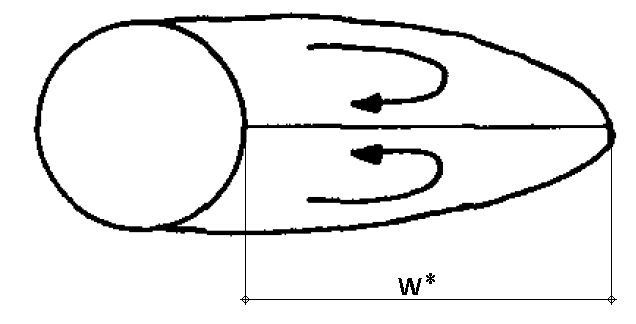
\includegraphics[height=4cm]{steadyFlow_modifiedWilliamson.PNG}
				\caption{Wake separation length \todo{Quelle modified!}}
				\label{fig:wakeSeparation}
			\end{figure} 
	It can be found from examining the velocity $U$ at $y=0$; the x-position where $U$ changes its sign should be the end position of the wake.
	\subsubsection{Simulation at Reynolds Number 10}

	\begin{figure}[htp]	
		\centering
		\begin{tikzpicture}
		\begin{semilogxaxis}[xlabel ={Cells per Direction}, ylabel ={$C_D$},  grid =major, legend entries ={$P=1$}, unbounded coords=jump, legend style = {cells = {anchor=east}, legend pos=outer north east,}, scaled x ticks = false, scaled y ticks = false, xmin = 32, xmax = 128, ymax = 2.7]
		\addplot table[ x = meshSize, y =C_D] {data/re10.dat};
		\addlegendentry{$P=1$}
		\addplot[mark=none, red] coordinates {(32, 2.5) (128, 2.5)};
		\addlegendentry{Constant Value}
		\end{semilogxaxis}	
		\end{tikzpicture}
		\label{shivfjfterror}	
		\caption{Convergence Plot}
	\end{figure}
	
	\begin{figure}[htp]	
		\centering
		\begin{tikzpicture}
		\begin{semilogxaxis}[xlabel ={Cells per Direction}, ylabel ={$C_L$},  grid =major, legend entries ={$P=1$}, unbounded coords=jump, legend style = {cells = {anchor=east}, legend pos=outer north east,}, scaled x ticks = false, scaled y ticks = false, xmin = 32, xmax = 128]
		\addplot table[ x = meshSize, y =C_L] {data/re10.dat};
		\addlegendentry{$P=1$}
		\addplot[mark=none, red] coordinates {(32, 0) (128, 0)};
		\addlegendentry{Constant Value}
		\end{semilogxaxis}	
		\end{tikzpicture}
		\label{shivfjftqerror}	
		\caption{Convergence Plot}
	\end{figure}

%	\begin{table}[htp]
%		\centering
%		\begin{tabular}{|c||c|c|c|c}
%			\cline{1-4}
%			\rule{0pt}{2,3ex}\multirow{2}{*}{}   & \multicolumn{3}{c|}{mesh size} &  \\ \cline{2-4}
%			\rule{0pt}{2,3ex}& $32 \times 32$       & $64 \times 64$       & $128 \times 128$      &  \\ \cline{1-4}
%			\rule{0pt}{2,3ex}$W^*$ 				 & a        & b        & c        &  \\ \cline{1-4}
%			\rule{0pt}{2,3ex}$C_D$                & $2.2763840026747$        & $2.3205402064175$        & $2.41364044322$        &  \\ \cline{1-4}
%			\rule{0pt}{2,3ex}$C_L$                & $-0.00055059425842785$        & $-0.0014617338683891$        & $0.00004720682$        &  \\ \cline{1-4}
%		\end{tabular}
%		\caption{Wake separation length and coefficients of drag and lift for $\text{Re}=10$}
%		\label{tab:re10}
%	\end{table}
	
	\subsubsection{Simulation at Reynolds Number 20}
	\begin{figure}[htp]	
		\centering
		\begin{tikzpicture}
		\begin{semilogxaxis}[xlabel ={Cells per Direction}, ylabel ={$C_D$},  grid =major, legend entries ={$P=1$}, unbounded coords=jump, legend style = {cells = {anchor=east}, legend pos=outer north east,}, scaled x ticks = false, scaled y ticks = false, xmin = 32, xmax = 128, ymax = 2.0]
		\addplot table[ x = meshSize, y =C_D] {data/re20.dat};
		\addlegendentry{$P=1$}
		\addplot[mark=none, red] coordinates {(32, 1.6) (128, 1.6)};
		\addlegendentry{Constant Value}
		\end{semilogxaxis}	
		\end{tikzpicture}
		\label{shivfjftersaror}	
		\caption{Convergence Plot}
	\end{figure}
\begin{table}[htp]
	\centering
	\label{my-label}
	\begin{tabular}{|c|l|c|c|c|}
		\hline
		\rule{0pt}{2,3ex}$\text{Re}=20$                              & Source                             & 2D/3D & $W^*$ & $C_D$ \\ \hline
		\rule{0pt}{2,3ex}\multirow{3}{*}{Numerical - Incompressible} & Dennis et al {[}1970{]}            & 2D    & 0.94     & 2.05     \\ \cline{2-5} 
		\rule{0pt}{2,3ex}& Forberg {[}1980{]}                 & 2D    & 0.91     & 2.00     \\ \cline{2-5} 
		\rule{0pt}{2,3ex}& Linnick et al. {[}2005{]}          & 2D    & 0.93     & 2.06     \\ \hline
		\rule{0pt}{2,3ex}\multirow{2}{*}{Experimental}               & Coutanceau et al. {[}1978{]}       & -     & 0.93    & -     \\ \cline{2-5} 
		\rule{0pt}{2,3ex}& Tritton {[}1959{]}                 & -     & -     & 2.09     \\ \hline
		\rule{0pt}{2,3ex}\multirow{3}{*}{Numerical Compressible}     & Brehm et al. {[}2015{]} (Ma = 0.1) & 3D    & 0.96     & 2.02     \\ \cline{2-5} 
		\rule{0pt}{2,3ex}& Ayers {[}2015{]}                   & 2D    & 0.975     & 2.06     \\ \cline{2-5} 
		\rule{0pt}{2,3ex}& \textbf{Present Results:}                   & 2D    & d     & 4     \\ \hline
	\end{tabular}	
	\caption{Comparison of Results for $W^*$ and $C_D$, \todo{modified Lawrence}}
\end{table}
	
%		\begin{table}[htp]
%			\centering
%			\begin{tabular}{|c||c|c|c|c}
%				\cline{1-4}
%				\rule{0pt}{2,3ex}\multirow{2}{*}{}   & \multicolumn{3}{c|}{mesh size} &  \\ \cline{2-4}
%				\rule{0pt}{2,3ex}& $32 \times 32$       & $64 \times 64$       & $128 \times 128$      &  \\ \cline{1-4}
%				\rule{0pt}{2,3ex}$W^*$ 				 & a        & b        & c        &  \\ \cline{1-4}
%				\rule{0pt}{2,3ex}$C_D$                & $1.64383538516091$        & $1.63699061840009$        & $1.63699061840009$       &  \\ \cline{1-4}
%				\rule{0pt}{2,3ex}$C_L$                & $-0.000776541603329406$       & $-0.000694847445600998$       & $-0.000694847445600998$        &  \\ \cline{1-4}
%			\end{tabular}
%			\caption{Wake separation length and coefficients of drag and lift for $\text{Re}=20$}
%			\label{tab:re20}
%		\end{table}
	\subsubsection{Simulation at Reynolds Number 40}
\begin{table}[htp]
	\centering
	\label{my-label}
	\begin{tabular}{|c|l|c|c|c|}
		\hline
		\rule{0pt}{2,3ex}$\text{Re}=40$                              & Source                             & 2D/3D & $W^*$ & $C_D$ \\ \hline
		\rule{0pt}{2,3ex}\multirow{3}{*}{Numerical - Incompressible} & Dennis et al {[}1970{]}            & 2D    & 2.35     & 1.52     \\ \cline{2-5} 
		\rule{0pt}{2,3ex}& Forberg {[}1980{]}                 & 2D    & 2.24     & 1.50    \\ \cline{2-5} 
		\rule{0pt}{2,3ex}& Linnick et al. {[}2005{]}          & 2D    & 2.28     & 1.54     \\ \hline
		\rule{0pt}{2,3ex}\multirow{2}{*}{Experimental}               & Coutanceau et al. {[}1978{]}       & -     & 2.13    & -     \\ \cline{2-5} 
		\rule{0pt}{2,3ex}& Tritton {[}1959{]}                 & -     & -     & 1.59     \\ \hline
		\rule{0pt}{2,3ex}\multirow{3}{*}{Numerical Compressible}     & Brehm et al. {[}2015{]} (Ma = 0.1) & 3D    & 2.26     & 1.51     \\ \cline{2-5} 
		\rule{0pt}{2,3ex}& Ayers {[}2015{]}                   & 2D    & 2.250     & 1.605     \\ \cline{2-5} 
		\rule{0pt}{2,3ex}& \textbf{Present Results:}                   & 2D    & d     & 4     \\ \hline
	\end{tabular}	
	\caption{Comparison of Results for $W^*$ and $C_D$, \todo{modified Lawrence}}
\end{table}
%		\begin{table}[htp]
%			\centering
%			\begin{tabular}{|c||c|c|c|c}
%				\cline{1-4}
%				\rule{0pt}{2,3ex}\multirow{2}{*}{}   & \multicolumn{3}{c|}{mesh size} &  \\ \cline{2-4}
%				\rule{0pt}{2,3ex}& $32 \times 32$       & $64 \times 64$       & $128 \times 128$      &  \\ \cline{1-4}
%				\rule{0pt}{2,3ex}$W^*$ 				 & a        & b        & c        &  \\ \cline{1-4}
%				\rule{0pt}{2,3ex}$C_D$                & $1.26492653340932$        & $1.20679001087588$        & $1.1891224168599$       &  \\ \cline{1-4}
%				\rule{0pt}{2,3ex}$C_L$                & $-0.000508760643668893$        & $-0.00157058413712008$        & $-0.00054056507571687$        &  \\ \cline{1-4}
%			\end{tabular}
%			\caption{Wake separation length and coefficients of drag and lift for $\text{Re}=40$}
%			\label{tab:re40}
%		\end{table}
	\subsection{Unsteady Simulations ($\text{Re}> 40-50$)}
	In order to compare the unsteady simulations we need the Strouhal number
	\begin{align}
		\text{St} = \dfrac{f  L_\infty}{V_\infty}.
	\end{align}
	As our initial and boundary conditions give $V_\infty = L_\infty = 1$, we can calculate $\text{St} = f$ with $f$ found from examining the oscillation of $C_L$ over time. 
	\subsubsection{Simulation at Reynolds Number 100}
\begin{table}[htp]
	\centering
	\label{my-label}
	\begin{tabular}{|c|p{4cm}|c|c|c|c|}
		\hline
		\rule{0pt}{2,3ex}$\text{Re}=100$                              & Source                             & 2D/3D & $St$ & $C_D$ & $C_L$\\ \hline
		\rule{0pt}{2,3ex}\multirow{7}{*}{Numerical - Incompressible} & Gresho et al. {[}1984{]}            & 2D    & 0.18     & 1.76 & -   \\ \cline{2-6} 
		\rule{0pt}{2,3ex}& Linnick et al. {[}2005{]} \newline ($\lambda = 0.056$)                 & 2D    & 0.169     & 1.38 \pm 0.010  &  \pm  0.337 \\ \cline{2-6} 
		\rule{0pt}{2,3ex}& Linnick et al. {[}2005{]} \newline ($\lambda = 0.023$)                  & 2D    & 0.169     & 1.34 \pm 0.009  &  \pm 0.333 \\ \cline{2-6} 
		\rule{0pt}{2,3ex}& Persillon et al. {[}1998{]}                 & 2D    & 0.165     & 1.253  & -  \\ \cline{2-6} 
		\rule{0pt}{2,3ex}& Saiki et al. {[}1996{]}                 & 2D    & 0.171     & 1.26  &  - \\ \cline{2-6} 
		\rule{0pt}{2,3ex}& Persillon et al. {[}1998{]}                 & 3D    & 0.164     & 1.240  & -  \\ \cline{2-6} 
		\rule{0pt}{2,3ex}& Liu et al. {[}1998{]}          & 3D    & 0.165     & 1.35 \pm 0.012  & \pm 0.339  \\ \hline
		\rule{0pt}{2,3ex}\multirow{2}{*}{Experimental}               & Berger et al. {[}1972{]}       & -     & 0.16-0.17    & -    & -\\ \cline{2-6} 
		\rule{0pt}{2,3ex}& Clift et al. {[}1978{]}                 & -    & -     & 1.24  &  - \\ \cline{2-6} 
		\rule{0pt}{2,3ex}& Williamson {[}1996{]}                 & -     & 0.164    & -   & - \\ \hline
		\rule{0pt}{2,3ex}\multirow{3}{*}{Numerical - Compressible}     & Brehm et al. {[}2015{]} \newline (Ma = 0.1) & 3D    & 0.165     & 1.32 \pm 0.01    & \pm 0.32 \\ \cline{2-6} 
		\rule{0pt}{2,3ex}& Ayers {[}2015{]}                   & 2D    & 0.167     & 1.371 \pm 0.011   & \pm 0.333 \\ \cline{2-6} 
		\rule{0pt}{2,3ex}& \textbf{Present Results:}                   & 2D    & d     & 4  &   \\ \hline
	\end{tabular}	
	\caption{Comparison of Results for $St$, $C_D$ and $C_L$, \todo{modified Lawrence}}
\end{table}
%			\begin{table}[htp]
%				\centering
%				\begin{tabular}{|c||c|c|c|c}
%					\cline{1-4}
%					\rule{0pt}{2,3ex}\multirow{2}{*}{}   & \multicolumn{3}{c|}{mesh size} &  \\ \cline{2-4}
%					\rule{0pt}{2,3ex}& $32 \times 32$       & $64 \times 64$       & $128 \times 128$      &  \\ \cline{1-4}
%					\rule{0pt}{2,3ex}$St$ 				 & a        & b        & c        &  \\ \cline{1-4}
%					\rule{0pt}{2,3ex}$C_D$                & d        & e        & f        &  \\ \cline{1-4}
%					\rule{0pt}{2,3ex}$C_L$                & g        & h        & i        &  \\ \cline{1-4}
%				\end{tabular}
%				\caption{Strouhal number and coefficients of drag and lift for $\text{Re}=100$}
%				\label{tab:re100}
%			\end{table}
				\begin{figure}[htp]	
					\centering
					\begin{tikzpicture}
					\begin{axis}[xlabel ={Time}, ylabel ={$C_L$}, grid =major, legend entries ={$P=1$}, unbounded coords=jump, legend style = {cells = {anchor=east}, legend pos=outer north east,}, scaled x ticks = false]
					\addplot table[ x =time  , y =C_L, mark=none] {data/vortex2.dat};
					\end{axis}	
					\end{tikzpicture}
					\label{shijftserdaror}	
					\caption{Convergence Plot}
				\end{figure}
			
				\begin{figure}[htp]	
					\centering
					\begin{tikzpicture}
					\begin{axis}[xlabel ={Time}, ylabel ={$C_L$}, grid =major, legend entries ={$P=1$}, unbounded coords=jump, legend style = {cells = {anchor=east}, legend pos=outer north east,}, scaled x ticks = false, xmin = 0, xmax = 120]
					\addplot table[ x =time, y =d, mark=none] {data/CLRE100.dat};
					\end{axis}	
					\end{tikzpicture}
					\label{shijfterror}	
					\caption{Convergence Plot}
				\end{figure}
				\begin{figure}[htp]	
					\centering
					\begin{tikzpicture}
					\begin{axis}[xlabel ={Time}, ylabel ={$C_L$}, grid =major, legend entries ={$P=1$}, unbounded coords=jump, legend style = {cells = {anchor=east}, legend pos=outer north east,}, scaled x ticks = false]
					\addplot table[ x =time, y =d, mark=none] {data/CLRE100.dat};
					\end{axis}	
					\end{tikzpicture}
					\label{shijfterror}	
					\caption{Convergence Plot}
				\end{figure}
				\begin{figure}[htp]	
					\centering
					\begin{tikzpicture}
					\begin{axis}[xlabel ={Time}, ylabel ={$C_L$},  grid =major, legend entries ={$P=1$}, unbounded coords=jump, legend style = {cells = {anchor=east}, legend pos=outer north east,}, scaled x ticks = false, scaled y ticks = false, xmin = 300, xmax = 350]
					\addplot table[ x =time, y =d, mark=none] {data/CLRE100.dat};
					\end{axis}	
					\end{tikzpicture}
					\label{shijfterror}	
					\caption{Convergence Plot}
				\end{figure}
	\subsubsection{Simulation at Reynolds Number 200}
\begin{table}[htp]
	\centering
	\label{my-label}
	\begin{tabular}{|c|l|c|c|c|c|}
		\hline
		\rule{0pt}{2,3ex}$\text{Re}=100$                              & Source                             & 2D/3D & $St$ & $C_D$ & $C_L$\\ \hline
		\rule{0pt}{2,3ex}\multirow{3}{*}{Numerical - Incompressible} & Dennis et al {[}1970{]}            & 2D    & 0.94     & 2.05 &    \\ \cline{2-6} 
		\rule{0pt}{2,3ex}& Forberg {[}1980{]}                 & 2D    & 0.91     & 2.00  &   \\ \cline{2-6} 
		\rule{0pt}{2,3ex}& Linnick et al. {[}2005{]}          & 2D    & 0.93     & 2.06  &   \\ \hline
		\rule{0pt}{2,3ex}\multirow{2}{*}{Experimental}               & Coutanceau et al. {[}1978{]}       & -     & 0.93    & -    & \\ \cline{2-6} 
		\rule{0pt}{2,3ex}& Tritton {[}1959{]}                 & -     & -     & 2.09   &  \\ \hline
		\rule{0pt}{2,3ex}\multirow{3}{*}{Numerical Compressible}     & Brehm et al. {[}2015{]} (Ma = 0.1) & 3D    & 0.96     & 2.02   &  \\ \cline{2-6} 
		\rule{0pt}{2,3ex}& Ayers {[}2015{]}                   & 2D    & 0.975     & 2.06   &  \\ \cline{2-6} 
		\rule{0pt}{2,3ex}& \textbf{Present Results:}                   & 2D    & d     & 4  &   \\ \hline
	\end{tabular}	
	\caption{Comparison of Results for $W^*$ and $C_D$, \todo{modified Lawrence}}
\end{table}
	
%			\begin{table}[htp]
%				\centering
%				\begin{tabular}{|c||c|c|c|c}
%					\cline{1-4}
%					\rule{0pt}{2,3ex}\multirow{2}{*}{}   & \multicolumn{3}{c|}{mesh size} &  \\ \cline{2-4}
%					\rule{0pt}{2,3ex}& $32 \times 32$       & $64 \times 64$       & $128 \times 128$      &  \\ \cline{1-4}
%					\rule{0pt}{2,3ex}$St$ 				 & a        & b        & c        &  \\ \cline{1-4}
%					\rule{0pt}{2,3ex}$C_D$                & d        & e        & f        &  \\ \cline{1-4}
%					\rule{0pt}{2,3ex}$C_L$                & g        & h        & i        &  \\ \cline{1-4}
%				\end{tabular}
%				\caption{Strouhal number and coefficients of drag and lift for $\text{Re}=200$}
%				\label{tab:re200}
%			\end{table}
			\begin{figure}[htp]	
				\centering
				\begin{tikzpicture}
				\begin{axis}[xlabel ={Time}, ylabel ={$C_L$}, grid =major, legend entries ={$P=1$}, unbounded coords=jump, legend style = {cells = {anchor=east}, legend pos=outer north east,}, scaled x ticks = false]
				\addplot table[ x =time, y =l, mark=none] {data/re200dg1.dat};
				\end{axis}	
				\end{tikzpicture}
				\label{shijfterdaror}	
				\caption{Convergence Plot}
			\end{figure}